\section{Evaluation of User Interfaces}\label{sec:evaluation}

Designing the user interfaces has been a gradual process throughout different
parts of the project.
To evaluate how well the process has gone, this section will evaluate on the
user interface based on user feedback discussed in Section~\ref{subsec:usability-tests},
and design heuristics that were used during the design phase as seen in Section~\ref{subsec:heuristics}.

During earlier parts of the design phase, the group quickly got a prototype of
the product up and running.
This was done to get early feedback before effort was put into polishing and completing features.
The feedback was useful and allowed the authors to narrow down the layout
and find alternatives to confusing design decisions.
The specific changes that have been made are the date picker, the diagram layout and that it was decided upon to remove
the arrow for navigating.

After more development, the product did now fulfill the requirements put forth
by NOVA, and the final user test was then planned with NOVA\@.
In the session, language selection was mentioned as a point of interest; some
guidance in terms of feature-explanations were also discussed.
More details can be seen in Section~\ref{subsubsec:user-test-2}.

The feedback gathered during the final test had some features out of
scope for the project, but others could be implemented with enough time.
%todo: Maybe specify if we want it to seem like we have fixed anything, or maybe remove.

To get a more objective evaluation, some heuristics have been a focus for
the user interface, and it is worth evaluating their effect on the final design.

\begin{figure}
    \centering
    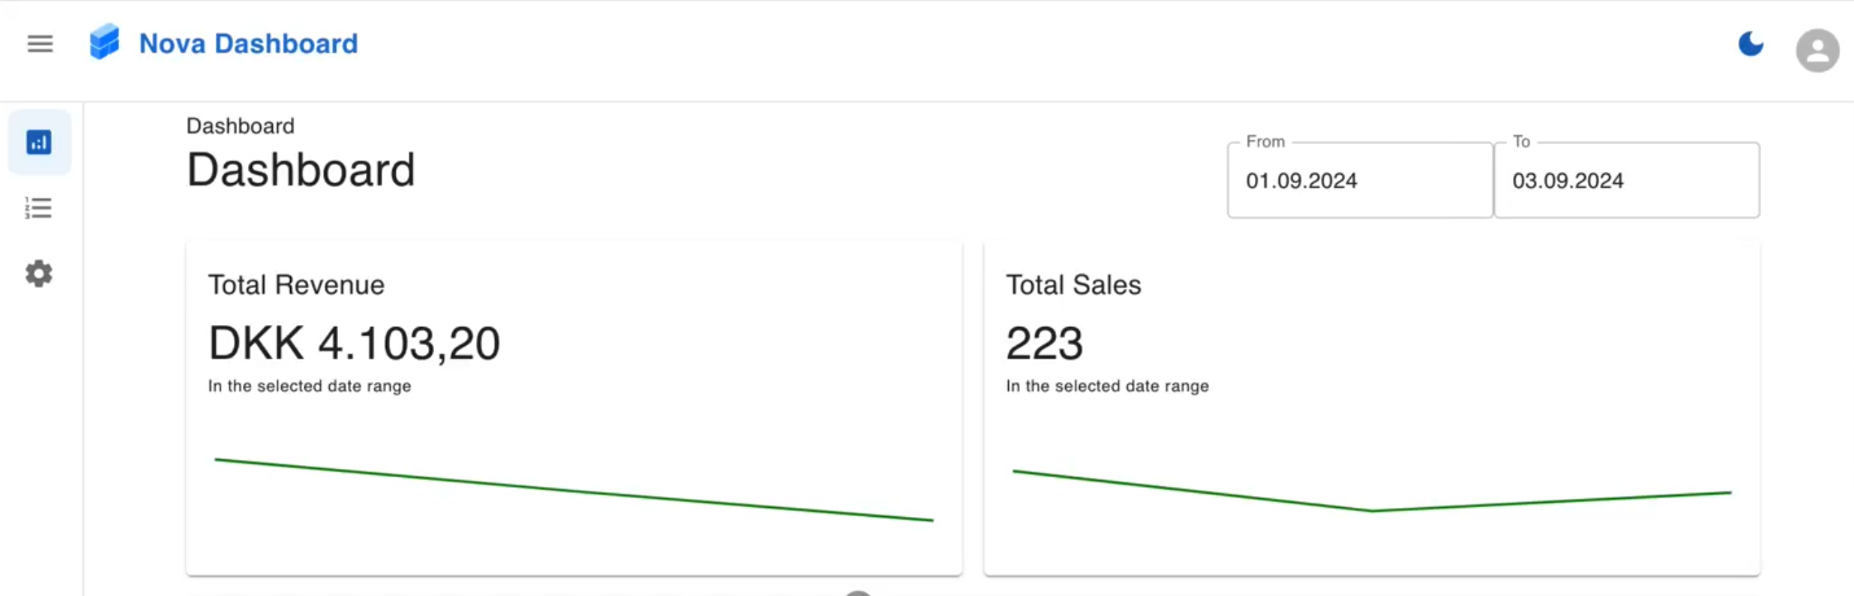
\includegraphics[width=\textwidth]{evaluation-heuristics}
    \caption{The final design of the header and sidebar.
    }\label{fig:evaluation-heuristics}
\end{figure}

The design seen in Figure~\ref{fig:evaluation-heuristics} is the final design
and different aspects of the design heuristics are at work.
In terms of design, a minimalist design with controlled colors works well
to give a sleek look, while letting the different components stand out.
To further improve the usability and easy of use, the design also follows
standard conventions by using a sidebar which acts as navigation for the site.
By using conventions, users do not have to search for standard features, and
can generally understand what the different components of the site do.
This has not been a complete success, as the user tests made clear that there
are issues.
The webpage also implements a date picker to dynamically render data to the user.
This is done to improve the flexibility and efficiency of use, and the effect
works well.
As was mentioned in Section~\ref{subsubsec:user-test-2}, a part of the site which
does not have the most efficient use is the data uploading.
This is discussed in Section~\ref{sec:future-development}, and is not something
that could be implemented in the final product.

For visibility of system status and error prevention, the site does this by using
notifications that inform the user of errors.
The minimalist design also works as error prevention, by only having necessary
interactions presented to the user.

Overall, the user interfaces succeed in letting the users work without interrupting
them, while having a simple design to keep the webpage focused.
